\documentclass{article}
\author{Victor Mittermair, 11809916}
\usepackage{hyperref}
\usepackage{fancyhdr}
\usepackage{tikz} 
\usepackage{amsthm}
\usepackage{verbatim}
\usepackage{subfigure}
\usepackage{amssymb}
\usepackage{mathtools}
\usepackage{amsmath}
\usepackage{soul}
\usepackage{algorithm}
\usepackage{algpseudocode}
\usepackage{algorithmicx}

\newtheorem*{theorem}{Theorem}
\newtheorem*{lemma}{Lemma}
\theoremstyle{definition}
\newtheorem*{definition}{Definition}
\theoremstyle{remark}
\newtheorem*{remark}{Remark}
\newtheorem*{note}{Note}
\newtheorem*{statement}{Statement}
\newtheorem*{example}{Example}

%\lhead{\includegraphics[width=0.2\textwidth]{nyush-logo.pdf}}
\fancypagestyle{firstpage}{%
  \lhead{TU Vienna}
  \rhead{
  Discrete Math for Informatics WS 2022}
}

%%%% PROJECT TITLE
\title{Discrete Math for Informatics\\
        \Large \emph{4th Lecture}}


\date{\today} %NO DATE



\begin{document}
\maketitle
\thispagestyle{firstpage}

\begin{comment}
\section*{Graph}
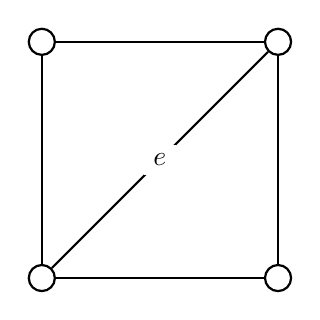
\begin{tikzpicture}[node distance={30mm}, thick, main/.style = {draw, circle}]
    \centering
    \node[main] (1)              {}; 
    \node[main] (2) [right of=1] {};
    \node[main] (3) [below of=1] {}; 
    \node[main] (4) [right of=3] {};
    \draw (1) -- (2) ; 
    \draw (1) -- (3); 
    \draw (2) -- (4); 
    \draw (3) -- (4);
    \draw (3) -- (2) node [midway, fill=white] {$e$}; 
\end{tikzpicture}

\end{comment}
\subsection*{How far do we have to go?}
$G$ a weighted directed graph $w: E \rightarrow \mathbb{R}$\\
Distance (or length) of a path P is $\sum_{e \in P} w(e)$ 
%graph 1
Algorithms:
\begin{itemize}
    \item \textbf{Dijkstra} (1950s) sinlge source, only for $w: \rightarrow \mathbb{R_+}$, $O(|V|log|V|+|E|)$
    \item \textbf{Bellman-Ford-Moore} single source, $G$ loopless, $O(|V||E|)$
    \item \textbf{Floyd-Warshall} all distances, $O(|V|^3)$
\end{itemize}

\begin{algorithm}
    Dijkstra algorithm: $d(v)$ (array of distances) $= 0 $ if $ v=v_0$ else $\infty$
    \begin{algorithmic}

    \State $Q \gets V$
    \While{$Q \neq \emptyset$}
        \State find $u \in Q$ with minimal $d(u)$
        \State $Q \gets Q \backslash u$
        \For{$v\in Q, (u,v) \in E$}
            \State $d(v) \gets min(d(v), d(u)+w(u,v))$
            \State (predecessor of $v$ is $u$ if $d(u) w(u,v) < d(v))$
        \EndFor
    \EndWhile
    \end{algorithmic}
\end{algorithm}
\begin{example}
    example 1
\end{example}
\begin{definition}
    A \textbf{cut} of a (di)graph is a set of edges(arcs) $S$ such that $V$ is the disjoint union of $V_1$ and $V_2$ and there is no edge within $V_1$ or $V_2$ in S\\
    graph 2
\end{definition}
\begin{remark}
    Dijkstra chooses the minmial weight edge between $Q$ and $V\backslash Q$, this is called \textbf{breadth-first search}
\end{remark}
\begin{algorithm}
    Bellman-For-Moore algorithm: $d(v)$ (array of distances) $= 0 $ if $ v=v_0 $ else $ \infty$
    $l(v)$ (length of path) $= 0 $ if $ v=v_0 $ else $ \infty$
    \begin{algorithmic}
    \State $step \gets 0$
    \While{True}
        \State $modified \gets False$
        \For{$u\in V$ with $l(u) = step$}
            \For{$e=(u,v) \in E$}
                \If{$d(v) > d(u) + w(e)$}
                    \State $modified \gets True$
                    \State $d(v) \gets d(u)+w(e)$
                    \State $l(v) \gets l(u)+1$
                \EndIf
            \EndFor
        \EndFor
        \If{not $modified$}
            \State \textbf{return} $d$
        \Else
            \If{$step = |V|-1$}
                \State throw error: negative cycle
            \Else 
                \State $step \gets step+1$
            \EndIf
        \EndIf
    \EndWhile
    \end{algorithmic}
\end{algorithm}
\begin{example}
    example 2
\end{example}
\begin{example}
    Of a negative cycle. graph 3
\end{example}
\begin{algorithm}
    Floyd-Warshall algorithm: $d(u,v)$ (array of distances) $= 0 $ if $ u=v $ else if $ (u,v) \in E$ $w(u,v)$ else $\infty$ (adjacency matrix with 0 replaced by $\infty$)
    \begin{algorithmic}
    \State $step \gets 0$
    \For{$u \in V$}
        \For{$v\in V$}
            \For{$w \in V$}
                \State $d(v,w) = min(d(v,w), d(v,u)+d(u,w)$)
            \EndFor
            \If{$d(v,v) < 0$}
                \State error: negative cycle
            \EndIf
        \EndFor
    \EndFor
    
    \end{algorithmic}
\end{algorithm}
\subsection*{Flows}
\begin{definition}
    $G$ a weighted (di)graph with $w: E \rightarrow \mathbb{R_+}$ $s$ a source in $V$, i.e indegree of $s$ is $0$ and $t$ a sink, i.e outdegree of $t $ is $0$.\\
    $\phi: E \rightarrow \mathbb{R}$ is a \textbf{flow} if:\\
    $F1:$ $\forall e \in E: 0 \leq \phi(e) \leq w(e)$\\
    $F2:$ $\forall v \in V\backslash \{s,t\} \sum_{(v,u)\in E} \phi(v,u)=\sum_{(u,v)\in E}\phi(u,v$)\\
    $val(\phi):=\sum_{(s,u) \in E}\phi(s,u)=\sum_{(u,t)\in E} \phi(u,t)$
\end{definition}
\begin{lemma}
    \begin{equation}
        \sum_{(s,u) \in E}\phi(s,u)=\sum_{(u,t)\in E} \phi(u,t)
    \end{equation}
\end{lemma}
\begin{proof}
    \begin{equation*}
        \sum_{(s,u) \in E}\phi(s,u) + \sum_{v\neq s,t; v \in V} \sum_{(v,u) \in E} \phi(v,u) = \sum_{e\in E} \phi(e) 
    \end{equation*}\\
    sum over outbound edges
    \begin{equation*}
    \sum_{(u,t)\in E} \phi(u,t) + \sum_{v\neq s,t; v \in V} \sum_{(u,v) \in E} \phi(u,v) = \sum_{e\in E}\phi(e)
    \end{equation*}\\
    sum over inbound edges
\end{proof}
graph 4
\end{document}